\documentclass[11pt]{article}
\usepackage[utf8]{inputenc}
\usepackage{graphicx}
\usepackage[italian]{babel}
\usepackage{hyperref}
\usepackage{float}
\title{Progetto di Tecnologie Web}


\begin{document}
	\maketitle
	\begin{figure}[h]
		\centering
		
\includegraphics[width=0.7\linewidth]{logo-unipd.png}
	\end{figure}
	\begin{center}{\fontsize{20}{10}\selectfont Autori:}\end{center}
	\begin{center}{\fontsize{20}{30}\selectfont 
			Walter Sandon 1009138
			Marco Casagrande 1049532
			}\end{center}
	
	\newpage
	\tableofcontents
	\newpage
	\listoffigures
	\newpage
	
\section{Informazioni Generali}

A questo progetto hanno lavorato due persone: Walter Sandon e Marco Casagrande.
Il referente del progetto, in quanto proponitore, è Walter Sandon.

L'idea del sito (descritta nell'Abstract appena sotto) è nata dall'esigenza di un suo amico che voleva rinnovare il sito internet della propria azienda, partendo da zero.

L'accesso alla zona riservata del sito è permesso soltanto con questa combinazione di dati:
Username: admin
Password: admin

Per condividere in tempo reale le modifiche, è stato utilizzato il sito \href{https://github.com/}.
Gli altri strumenti utilizzati, specialmente i validatori, verranno citati nelle apposite sezioni.

\section{Abstract}

Il progetto sviluppato implementa il sito internet di una azienda che produce per conto terzi griglie metalliche ad uso domestico (per forni, frigoriferi e simili).
Il sito si propone di fornire in modo elegante, rapido e efficace ogni informazione riguardante la IMAS: specialmente i prodotti offerti e le relative lavorazioni disponibili, la posizione geografica ed i contatti per comunicare con la ditta.
Quest'ultimi sono di particolare importanza, in quando lo scopo principale del sito non è vendere prodotti ad un prezzo prefissato, ma stringere accordi commerciali di fornitura con altre aziende.
Inoltre, gli amministratori hanno la possibilità di accedere ad un area riservata che offre le seguenti funzionalità:
\begin{itemize}
	\item inserire un nuovo prodotto,
	\item modificare un prodotto esistente,
	\item eliminare un prodotto esistente,
	\item inserire una nuova lavorazione,
	\item modificare una lavorazione esistente,
	\item eliminare una lavorazione esistente,
	\item assegnare a più prodotti una lavorazione esistente.
\end{itemize}
Tutto questo deve avvenire in modo automatico e controllato.
 
\newpage
\section{Utenti destinatari}

\paragraph{Aziende}
La prima e più importante categoria di utenti destinatari comprende le aziende.
Vista l'orientamento commerciale del sito, è naturale che le aziende coinvolte nelle categorie merceologiche della IMAS sia interessate ai loro \textit{Prodotti}.\\
Questi utenti potranno visualizzare il catalogo dei prodotti che recano una descrizione e l'elenco delle possibili \textit{lavorazioni}, che potranno essere approfondite nell'apposita sezione.\\
Per queste aziende è stata sviluppata la sezione \textit{Contatti} affinchè abbiano i mezzi più semplici e veloci possibili per comunicare con la IMAS.\\
Inoltre la sezione \textit{Home} si pone l'obbiettivo di dimostrare l'affidabilità e la filosofia aziendale, così da trasmettere sempre un'opinione positiva agli utenti.

\paragraph{Amministratori}
Una seconda categoria di utenti del sito è rappresentata dagli amministratori IMAS. Essi possono accedere, autenticandosi attraverso un link nell' \textit{header} a destra del logo aziendale, ad un'area riservata dalla quale è possibile gestire i prodotti e le lavorazioni offerti dalla ditta.

\paragraph{Privati}
L'ultima categoria comprende genericamente i privati. Nonostante non abbiano la stessa rilevanza economica di un'azienda, questi utenti sono comunque incoraggiati a visitare il sito che fornisce utili informazioni consultabili anche da chi non è pratico del settore.

\newpage
\section{Usabilità}

Dopo aver discusso col proponente riguardo alle possibili implementazioni del sito, si è passati nella fase di progettazione.
La questione principale è stata il come distribuire le varie informazioni nel sito, cercando di collocarle tutte in modo chiaro ed ordinato.
Si è arrivati alla conclusione che le due azioni principali degli utenti siano due:
\begin{description}
	\item [Consultare il catalogo prodotti] \hfill \\
	L'operazione più frequentemente compiuta dagli utenti è quella di consultare il catalogo dei prodotti presenti.
	\\
	Essendo però una ditta che non ha una continuità di rinnovo dei prodotti, si è ritenuto opportuno non metterlo in evidenza nella \textit{Home}, ma piuttosto dedicare un area apposita.
	La \textbf{Home} ha lo scopo di accogliere ed informare gli utenti nuovi riguardo alle origini, alla storia a alla mission aziendale. In generale si vuole attirare il visitatore e lasciargli un'impressione favorevole della IMAS anche in caso non fosse interessato.\\
	Per facilitare gli spostamenti all'interno del sito è stata inoltre predisposta una comoda \textit{NavBar} con la quale raggiungere le quattro sezioni pubbliche cioè \textbf{Home}, \textbf{Prodotti},\textbf{Lavorazioni} e \textbf{Contatti}.

	\item [Manutenzione del catalogo] \hfill \\
	L'operazione di manutenzione dei cataloghi(cioè la gestione dei prodotti e delle lavorazioni) è riservata agli amministratori del sito.\\
	 È logico pensare che, essendo tali utenti un numero inferiore rispetto ai visitatori, il link per l'autenticazione e l'accesso all'area riservata possa essere messa in posizione \textit{nascosta}. Purtroppo per ragioni di spazio, è stata semplicemente posizionata in alto a destra sapendo di creare così disorientamento per gli altri utenti ignari.\\
	 Abbiamo cercato di limitare i danni avvisando,  una volta entrati nell'area login, che tale area è riservata ai dipendenti IMAS.\\
	  \textit{Si noti che l'accesso all'area di amministrazione è visibile solo dopo aver effettuato il login.}
\end{description}

\subsection{Elementi dell'Interfaccia Grafica}

Per rendere l'infertafaccia il più chiara (intuitiva per ogni utente) e diretta (minor numero di click per un operazione) possibile, sono stati impiegati i seguenti elementi:
\begin{description}
	\item [NavBar] La barra di navigazione è presente in ogni pagina e consente l'accesso diretto alle 4 sezioni pubbliche \textit{Home}, \textit{Prodotti}, \textit{Lavorazioni} e \textit{Contatti}.
	\\È stata progettata in modo tale che l'utente sappia in ogni momento in che pagina si trova. Infatti la parte della barra corrispondente alla pagina visitata risulta essere evidenziata.
	\item [Breadcrumbs] Fornisce una semplice mappa del sito, segnalando il percorso dalla \textit{Home} alle sezioni più interne del sito. Per un miglior orientamento, il colore corrisponde a quello attribuito alla sezione corrente (ritrovabile nella \textit{NavBar}.
	\item [Link] Abbiamo deciso di adottare due tipologie di link, quelli che si trovano immersi nel testo e quelli che invece sono inseriti nelle due sezioni precedentemente descritte.
	\\ I primi sono sottolineati e aderiscono alla rappresentazione standard dei link ovvero blu se non visitati e viola in caso contrario. I secondi, più simili a pulsanti, sono ben visibili poichè cambiano di colore al passaggio del mouse.
\end{description}

\newpage
\section{Gerarchia file}

La gerarchia del sito è organizzata in 3 cartelle:
\begin{itemize}
	\item \texttt{cgi-bin} con gli script \texttt{.cgi}
	\item \texttt{data} con 3 sotto-cartelle
	\begin{itemize}
		\item \texttt{xml} contenente tutti i file XML
		\item \texttt{xsd} contenente gli \textit{XMLSchema}
		\item \texttt{xsl} contenente i fogli di trasformazione
	\end{itemize}
	\item \texttt{public\_html} con il file \texttt{index.html} e le sotto-cartelle:
	\begin{itemize}
		\item \texttt{images} con le immagini che ci sono servite per decorare il sito
		\item \texttt{icons} con la favicon per la tab del browser
		\item \texttt{javascript} con le funzioni scritte in \textit{JavaScript}
		\item \texttt{parts} con i file xhtml parziali, ovvero parti di codice xhtml che verranno stampate dinamicamente grazie al Perl
		\item \texttt{css} con i fogli di stile  
	\end{itemize}
\end{itemize}

\newpage
\section{Architettura}

\subsection{Progettazione layout}

Prima di iniziare la stesura del codice abbiamo cercato di organizzare i dati che volevamo rappresentare. Questo ci ha permesso di chiarire alcuni aspetti fondamentali del sito. Innanzitutto la semplicità di navigazione al suo interno: se un sito è semplice è visitabile ed usufruibile da più persone. Ciò non toglie che il visitatore di IMAS difficilmente ci sarà arrivato per caso, ma più realisticamente avrà effettuato una ricerca molto specifica. Dunque si può presupporre un minimo livello di conoscenza della navigazione web.
\\
\\
Fin da subito abbiamo optato per un layout di tipo fluido. Ha richiesto più lavoro del previsto in quanto era necessario adattarlo ai vari tipi di monitor cambiando di molto l'aspetto, ma questo ha reso possibile un alto indice di accessibilità.

\subsection{Sviluppo layout}

Nell'immagine sottostante è possibile visualizzare la struttura principale dei div, i quali raccolgono per contenuto tematico le informazioni.
Il layout adottato ha come larghezza massima 1200px dovuto ad un fattore estetico dato che le varie sezioni del \textit{Container} cambiano di lunghezza ad ogni cambio d'informazione, mentre l'altezza non è stata in nessun modo alterata rispetto l'originale. Questo permette una evoluzione verso il basso senza problemi.
\begin{figure}[H]	
	\centering
	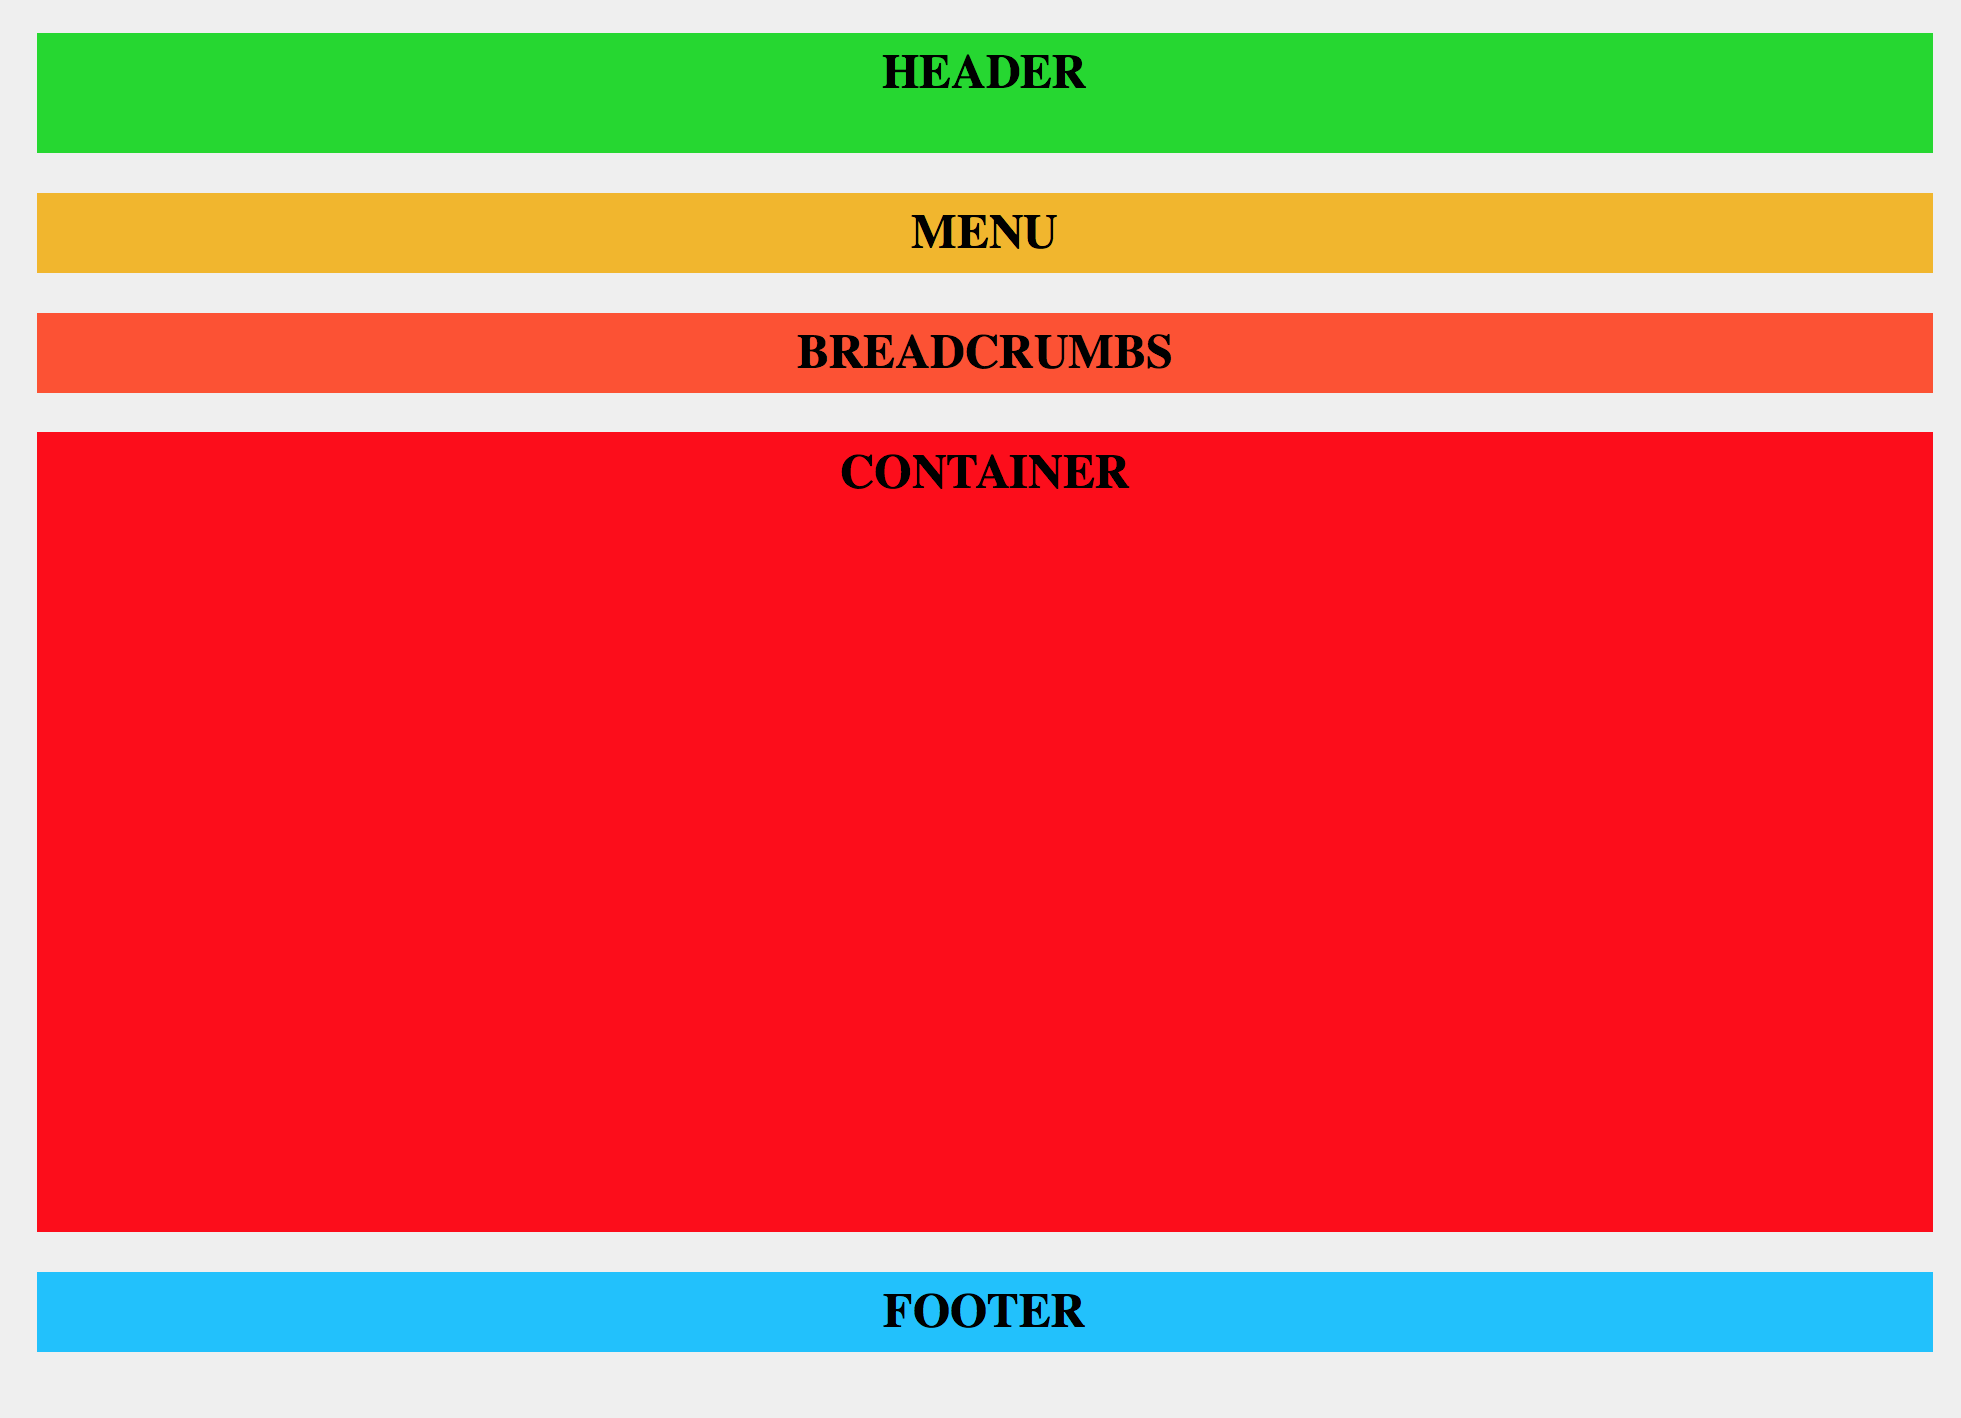
\includegraphics[width=\linewidth]{layout.png}
	\caption{Layout delle pagine}
	\label{Layout delle pagine}
\end{figure}

Visto il nostro target d'utenza, cioè le aziende,  si è deciso di puntare ad un layout adatto a portatili piuttosto che a schermi di grandi dimensioni. Non è stata sviluppata la parte mobile lato smartphone, tuttavia sono stati garantiti contenuti privi di alterazioni spiacevoli almeno fino a quando alla grandezza dello schermo dei tablet in modalità portrait. 
\\
\\
L'intero layout è stato progettato a pannelli adattabili, così da godere di maggiore espandibilità.
\begin{itemize}
	\item Partendo con l'analisi dall'alto si evidenzia subito il div "header" con il compito di informare l'utente su ciò che sta visitando.
	\\In questo caso siamo stati un po' condizionati dal fatto di non avere una totale libertà. Infatti manca una breve descrizione per far capire all'utente quale sia la tematica del sito.
	\\Come trattato in precedenza a lato a destra è presente il link per l'accesso agli amministratori.
	\item Sempre nell'area di maggior visibilità è presente il menu utente. Anch'esso è stato identificato tramite l'utilizzo del div "menu". Presenta 4 campi rappresentati da \textbf{Home}, \textbf{Prodotti}, \textbf{Lavorazioni} e \textbf{Contatti}. Evidenzia il menù attivo in ogni pagina del sito. E' l'asse informativo delle possibili sezioni visitabili.
	\item Sottostante il menu principale è presente il div "breadcrumbs". Ha il compito di aiutare l'utente a capire dove si trovi rispetto alla \textit{Home}. E' l'asse informativo per la localizzazione della posizione attuale.
	\item Il blocco centrale è rappresentato dal div "container". Ha il compito di raccogliere la sezione principale, tutte le informazioni che verranno esposte ai visitatoro compaiono qui. E' l'asse informativo dell'argomento trattato.
	\item Nella parte inferiore del sito è stato creato il div "footer", al suo interno sono presenti le credenziali della ditta e i loghi della certificazione html e css.
\end{itemize}

\subsection{Layout per dispositivi mobile}

Il layout per i dispositivi mobile è stato sviluppato per risoluzioni non inferiori ai 768px. L'aspetto del sito non varia, ma si è cercato di ridimensionare i font piuttosto che la grandezza delle immagine in modo da utilizzare quanta più area possibile per la visualizzazione.
\\Ove non è stato possibile è stata cambiata la disposizione degli elementi.

\subsection{Layout di stampa}

Nel layout di stampa si è deciso di eliminare tutte le informazioni superficiali e di mantenere il contenuto semplice e privo di colori e in parte di immagini. Vista la natura commerciale del sito, si vuole offrire una stampa che riporti solo le informazioni chiave all'utente. In particolare, saranno le sezioni Prodotti e Lavorazioni ad essere oggetti di stampa, che infatti riportano le immagini dei vari prodotti ed una lista di rapida consultazione. 
\\Le sezioni amministrative mantengono lo stesso stile minimale, considerato anche lo scarso interesse nello stamparle. Nel layout di stampa si è cercato di non modificare i font rispetto a quelli di default, in modo da non alterare la relativa qualità di stampa o la portabilità nel caso di stampa in PDF.

\newpage
\section{Struttura}

La struttura del sito è stata suddivisa per contenuti, in modo da aiutare l'utente nella ricerca delle informazioni. Questo porta ad una maggiore chiarezza delle sezioni presenti.
\\
\\
Tutto il sito è stato sviluppato in XHTML 1.0 Strict. Le pagine sono generate da Perl tramite sistemi di templating. L'unica eccezione riguarda la pagina Contatti, che necessitava di alcuni elementi di HTML5.
\\
\\Le pagine principali sono:
\\
\begin{description}
	\item[public\_html/index.html] \hfill \\
	 tramite l'utilizzo della funzione \textit{http-equiv="refresh"} abbiamo reso possibile il reindirizzamento alla \textit{Home} che si trova all’interno della cartella "cgi-bin", nel caso l'utente acceda alla directory principale del sito;
	 \item[cgi-bin/index.cgi]  la pagina viene generata con un contenuto esclusivamente statico richiamando altre parti comuni e specifiche della pagina che si trovano in \textbf{public\_html/parts}. La parte comune in ogni pagina risulta essere solo il footer, mentre l'header ed il menu, se pur considerati statici, sono specifici alla pagina;
	 \item[cgi-bin/prodotti.cgi]  questa pagina viene generata da un contenuto sia dinamico che statico. Dove la parte statica è formata dall'header, menu e footer, mentre il contenuto presente nel \textit{container} è generato dinamicamente richiamando "../data/xsl/prodotti.xslt" che estrae dall'xml i dati necessari per la composizione della pagina;
	 \item[cgi-bin/lavorazioni.cgi]  come per la pagina precedente, anch'essa è composta sia da contenuto statico che dinamico. La parte dinamica si differenzia dal fatto che non viene richiamato lo stesso file \textit{.xslt} ma quello specifico delle lavorazioni. 
	 \item[cgi-bin/contatti.cgi] questa pagina è costruita similmente alla \textit{Home} in quanto il suo contenuto è totalmente statico. La particolarità di questa pagina è che richiama del codice Javascript contenuto in \textit{public\_html/javascript} per inviare un'email preformattata tramite il tasto \textbf{invia}.
	 \\La pagina offre degli aiuti nel caso si inseriscano dei dati errati;
	 \item[cgi-bin/login.cg] la seguente pagina permette l'autenticazione degli amministratori per poter accedere all'area riservata, emettendo se necessario un messaggio di errore.
	 \\Dal momento in cui ci si logghi in ogni pagina al posto del link \textit{Area Riservata} saranno presenti 2 link per l'area \textbf{Amministrazione}e per il \textbf{Logout};
	 \item[cgi-bin/admin.cg] è l'hub per la gestione dei prodotti e delle lavorazioni. Tramite queste due sezioni si può accedere ad una delle varie operazioni disponibili.
\end{description}
\newpage

\section{Presentazione}

Per la presentazione delle informazioni abbiamo cercato di essere quanto più precisi possibili ed accessibili. Abbiamo deciso di sviluppare l'interfaccia grafica tramite l'utilizzo di codice CSS, che è stato correttamente validato nella versione CSS3.
\\
Tutte le pagine mostrano una grafica diversa, simili solo nell'alternanza del colore al cambio informazione. Questo è stato necessario in quanto ogni pagina presenta un aspetto diverso non compatibile semanticamente con quello delle altre pagine.
\\ E' stato definito un design accattivante e piacevole alla vista che però risulta a volte prolisso. 
\\
Per migliorare la presentazione e le performance, i file CSS sono stati divisi in base alle funzioni a loro riservate. Esistono 3 file CSS:
\begin{itemize}
	\item Il file "default.css" utilizzato per la maggior parte dei dispositivi con risoluzione maggiore.
	\item Il file "mobile.css" utilizzato per la parte dei dispositivi mobili quali i tablet, dove la dimensione dello schermo rimane più compatta. Esso viene attivato ad una risoluzione inferiore ai 768px.
	\item Il file "print.css" utilizzato per la stampa delle pagine.
\end{itemize}

La struttura della zona di amministrazione, avendo aree molto simili tra loro (es: inserimento prodotto e lavorazione), permette il riutilizzo di layout con variazioni minime così da favorire l'orientamente dell'utente. Inoltre, sono state frequentemente riutilizzate alcune classi (es: textbold, formmargin) così da facilitare un'eventuale estensione del sito. 
A questo scopo, sono stati posti alcuni commenti per indicare l'area di influenza delle varie classi.

\subsection{Combinazione dei colori}

Per cercare di garantire una totale usabilità del sito anche ad utenti affetti da problemi visivi è stato scelto uno schema a colori prevalentemente grigio che pure si adatta tematicamente ai prodotti in metallo.

Tutte le immagini impiegate sono state testate tramite il servizio offerto da \href{http://www.color-blindness.com/coblis-color-blindness-simulator/} e sono risultate chiaramente visibili.

Gli unici colori che potrebbero apparire poco chiari agli utenti con deficit visivi sono quelli del \textit{NavBar}, tuttavia restano distinguibili tra di loro e dunque si ritiene non pongano veri problemi.

A seguire alcune immagini estratte dal sito per dimostrarne l'aspetto:

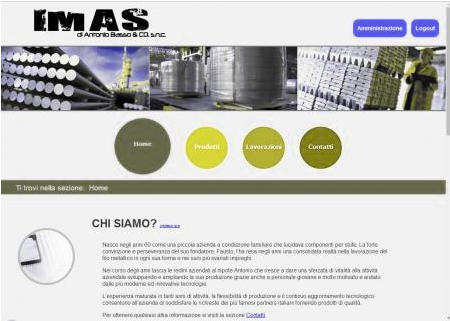
\includegraphics[width=0.3\textwidth]{HomeP.png}
\caption{Home Protanopia}
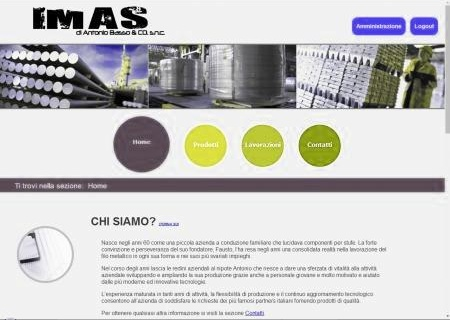
\includegraphics[width=0.3\textwidth]{HomeD.jpg}
\caption{Home Deuteranopia}
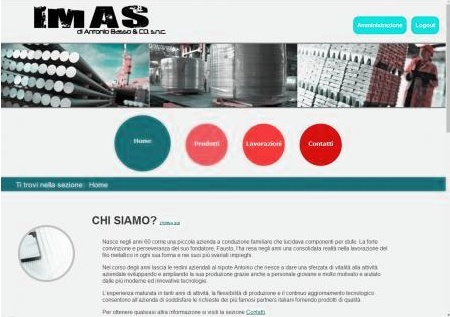
\includegraphics[width=0.3\textwidth]{HomeT.jpg}
\caption{Home Tritanopia}

\includegraphics[width=0.3\textwidth]{ProdottiP.jpg}
\caption{Prodotti Protanopia}
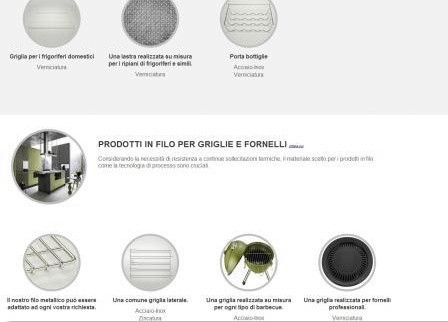
\includegraphics[width=0.3\textwidth]{ProdottiD.jpg}
\caption{Prodotti Deuteranopia}
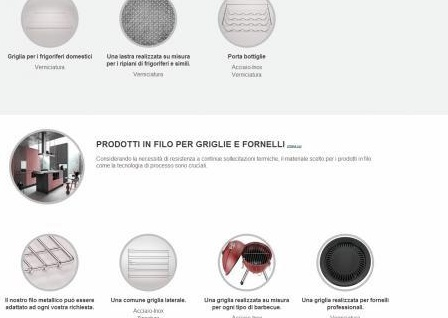
\includegraphics[width=0.3\textwidth]{ProdottiT.jpg}
\caption{Prodotti Tritanopia}

Il font utilizzato è di tipo standard e tutti i caratteri hanno una dimensione relativa, permettendo così una maggiore adattabilità alle preferenze dell'utente, senza influire negativamente nell'aspetto del sito.

\newpage
\section{Gestione dati}
Tutti i dati sono immagazzinati nei file xml.
\begin{description}
	\item[Login.xml]\hfill \\
	È l'elenco delle combinazioni "username" + "password" che possono accedere alla zona di amministrazione del sito.
	I nodi che scrivono le caratteristiche delle categorie sono:
	\begin{itemize}
		\item username
		\item password
	\end{itemize}
	\item[Prodotti.xml] \hfill\\È l'elenco dei prodotti disponibili e sono divisi in 3 categorie prefissate.
	I nodi che scrivono le caratteristiche delle categorie sono:
	\begin{itemize}
		\item nome
		\item foto
		\item attributo alt della foto
		\item descrizione
		\item prodotto
	\end{itemize}
	Ogni categoria può avere zero o più prodotti.
	I nodi che descrivono le caratteristiche dei prodotti sono:
	\begin{itemize}
		\item ID
		\item nome
		\item foto
		\item attributo alt della foto
		\item descrizione
		\item lavorazione
	\end{itemize}
	Ogni prodotto può essere disponibile sotto zero o più lavorazioni.
	\item[Lavorazioni.xml]\hfill \\ È l'elenco delle lavorazioni disponibili. 
	I nodi che descrivono le caratteristiche delle lavorazioni sono:
	\begin{itemize}
		\item nome
		\item attributo produzione
		\item foto
		\item attributo alt della foto
		\item descrizione
		\item commento
	\end{itemize}
\end{description}
Le funzionalità per la gestione dei dati sono offerte con controlli automatici nel sito, così che possano essere sfruttare da utenti inesperti.

\newpage
\section{Comportamento}
Il comportamento del sito è regolato da controlli sia da parte del Perl, sia di Javascript.

Riguardo al primo, verrà approfondito nella sezione successiva e coinvolge solo gli utenti amministratori. Il Perl si occupa della gestione dei dati immagazzinati nei file xml.

\subsection{Javascript}

L'unico script Javascript nella sezione \textit{Contatti}, dove gli utenti possono usufruire di un modulo per compilare automaticamente un'email con i loro dati personali, la categoria della richiesta e la descrizione. I controlli sono eseguiti sulla correttezza dei dati immessi (campi obbligatori, formato dell'email, lunghezza messaggio) e vengono effettuati all'invio della richiesta, segnalando se necessario luogo e motivo dell'errore.

Nel caso l'utente abbia disabilitato Javascript, non potrà usufruire della precompilazione del modulo, ma potrà comunque scrivere un'email nella maniera classica.

\subsection{Perl}

Il linguaggio Perl è stato utilizzato sia per stampare modularmente e dinamicamente le varie pagine, sia per il corretto funzionamento dei servizi offerti dal sito, cioè il login e la gestione dei prodotti e delle lavorazioni.
\\Le librerie utilizzate sono state:

\begin{itemize}
	\item CGI
	\item Lib::XML
	\item Lib::XSLT
\end{itemize}

Riguardo alla stampa delle pagine, si è sfruttata una combinazione di print e pagine xhtml così da produrre l'output opportuno.
\\Riguardo al login, tramite l'apposito form il Perl controlla in login.xml se l'username e la password corrispondano, restituendo un errore oppure permettendo l'accesso alla zona di amministrazione. Solo i gestori del sito hanno accesso a quest'area e non vi è modo di registrarsi. 
SI ricorda che l'unica combinazione di dati accettata è:
Username: "admin"
Password: "admin"
Nel caso si volesse registrare un nuovo amministrazione, è necessario intervenire direttamente in login.xml.

Il login inoltre crea una sessione tramite CGI::Session.
In questo modo ogni area della zona di amministrazione controlla se chi vi accede sia loggato o meno, e nel caso di risposta è negativa si attiva il reindirizzamento a login.cgi.

Riguardo alla gestione dei prodotti e delle lavorazioni, vengono offerte 5 funzionalità per chi non è pratico di XML che garantiscono il rispetto del corrispondente XMLSchema.

Queste funzionalità si possono suddividere in due categorie dal codice molto simile:

\begin{description}
	\item[Inserimento] alla quale appartengono l'inserimento prodotto/lavorazione. Questa categoria crea un nodo con i parametri impostati dall'amministratore, lo controlla e lo inserisce nel rispettivo file XML.
	\item[Modifica] alla quale appartengono la modifica prodotto/lavorazione e la riassegnazione di una lavorazione ai diversi prodotti.
	Questa categoria si occupa di modificare od eliminare i nodi in base alle scelte dell'amministratore. Inizialmente occorre selezionare l'elemento, poi verrà mostrata la pagina con i parametri modificabili. I cambiamenti vengono controllati ed introdotti nei rispettivi file XML.
\end{description}

Alcuni dettagli degni di nota sono:
\begin{description}
	\item Inserire un nuovo prodotto gli assegna automaticamente un ID unico
	\item Qualsiasi errore nella gestione blocca il codice prima che avvengano cambiamenti
	\item Inserire una nuova immagine comporta la cancellazione di quella vecchia
	\item La maggior parte dei campi dati attingono ai valori direttamente dal corrispondente file XML
	\item I campi dati vuoti delle modifiche possono essere semplicemente lasciati in bianco così da lasciare inalterato il loro valore
	\item La principale ragione d'essere della funzionalità di riattribuzione di una lavorazione ai vari prodotti, è semplificare l'aggiornamento dei prodotti dopo l'inserimento di una nuova lavorazione (altrimenti sarebbe necessario modificare ogni singolo prodotto aggiungendo la lavorazione)
	\item Si possono avere due prodotti con lo stesso nome dato che la loro chiave è l'ID, mentre due lavorazioni non possono avere lo stesso nome (ciò è garantito da un controllo automatico)
\end

\newpage
\section{Validazione}

Tutte le aree del sito sono state validate tramite \href{https://validator.w3.org/}.
Nessuna ha segnalato alcun avvertimento od errore con XHTML 1.0 Strict (o HTML5 per la sezione Contatti).

I 3 file CSS (default, mobile e print) sono stati validati tramite il sito \href{https://jigsaw.w3.org/css-validator/}.
Con la versione CSS3 nessuno ha segnalato alcun avvertimento od errore.
Avendo usato elementi come "border-radius" ovviamente la versione CSS2.1 segnala errore.

XML ed XMLSchema sono stati validati tramite \href{http://www.utilities-online.info/xsdvalidation/}.
Sia i file XML che quelli XMLSchema sono risultati ben formati, ed anche la validazione tra loro ha avuto un esito positivo.

Per testare e valutare il corretto sviluppo della trasformazione XSLT in modo rapido è stato utilizzato \href{http://www.w3schools.com/xsl/tryxslt.asp?xmlfile=cdcatalog&xsltfile=tryxsl_if}.

Si è cercato, almeno in parte vista l'impossibilità di un'automatizzazione completa, di valutare l'accessibilità tramite \href{http://achecker.ca/checker/index.php}. 
Questo strumento rileva i problemi attuali e potenziali secondo le linee guide del WCAG 2.0 (Level AA). 
Data l'importanza delle 4 sezioni pubbliche, si è testato il codice di Home, Prodotti, Lavorazioni e Contatti. Non è stato evidenziato alcun problema serio, ma solo potenziale (anche se in gran numero), lo si ritiene dunque un risultato soddisfacente.

Il sito è stato visualizzato dai browser
\begin
	\item[Google Chrome] versione 49.0.2623.112 m (da Windows Vista)
	\item[Internet Explorer] versione 9.0.8112.16421 (da Windows Vista)
	\item[Firefox] versione 43.0.4 (da Windows Vista)
\end

Non si è rilevato alcun problema critico di compatibilità tra queste piattaforme e quindi il risultato è stato giudicato soddisfacente.

\end{document}
